\section{Limitations}

Through our paper, we evaluate vanilla and recurrent-depth transformers on a single family of implicit reasoning problems. While we cleanly isolate systematic generalization and depth exploration in compositional reasoning, we do not cover the entire range of reasoning problems relevant to modern language models \citep{huang2023towards}. In order to maintain a controlled setting and properly study the behavior of recurrent-depth models, our experiments are intentionally small-scale and focused. This potentially limits direct extrapolation of results to modern LLMs whose performance and behavior is shaped by many additional factors like tokenizer choices, heterogeneous internet-scale data, pretraining data, post-training procedures and optimization at a much larger scale. Althought we study somewhat larger models in Appendix~\ref{app:ratios}, these are still significantly limited in scale relative to frontier LLMs today.

Additionally, our task formulation abstracts away many aspects of real-world language use. Inputs are presented in a highly structured form with dedicated entity and relation tokens with a very limited vocabulary. This removes challenges that might arise from surface-form variation, underspecification, distractor information, and distribution shift in natural language. Therefore, we do not claim complete and immediate transfer of positive results to LLMs trained with recurrent-depth at scale. However, we hope to isolate architectural effects in a controlled setting and use them to inform future designs for more robust implicit reasoning in future LLMs.

\section{Dataset}
\label{app:permutation}
To investigate how our implicit reasoning models scale to deeper $k$-hop composition tasks, we design a dataset from a permutation-based knowledge graph. In this setup, we found that models can sometimes achieve high accuracy via \emph{shortcuts} rather than performing the intended multi-step traversal. For large $k$, the final tail entity $t$ can become nearly determined by a short suffix of the relation sequence. Thus, a model may learn a shallow mapping from the trailing relations to the answer instead of retrieving the intermediate entities. To overcome this, We first construct a set of atomic facts over $|E|=200$ entities and $|R|=10$ relations. For each relation $r \in R$, we sample a random permutation $\pi_r$ over the entity indices and define the atomic facts as
\[
\forall e_i \in E:\quad (e_i, r, e_{\pi_r(i)}).
\]
Thus, each relation acts as a bijection over the entity set. Since the out-degree is set to $d=|R|=10$, every entity has exactly one outgoing edge for each relation. This ensures that each relation has full coverage over entities. To generate a $k$-hop example, we sample a starting atomic fact and then iteratively extend it by following outgoing edges from the current tail entity. At each step, one outgoing relation-edge pair is selected uniformly at random. Intermediate entities are used only during construction and are not included in the final training example. 

% We generate datasets for hop lengths $k \in [2,40]$. For each hop length, we construct 15,750 unique examples, which are then randomly split into 15,000 training examples and 750 test examples. This construction yields a controlled multi-hop compositional reasoning dataset in which each atomic relation is deterministic and globally defined over the full entity set, while longer-hop examples require repeated composition of these relation mappings.  In our setup, composing relations corresponds to composing permutations encouraging reliance on the entire relation sequence and retrieval of each intermediate entity.


\section{Training details and additional parameters}\label{app:training}

For most experiments, we use an embedding dimension of 768, 12 attention heads and a recurrent block of 4 transformer layers. However, in Appendix~\ref{app:ratios} we experiment with recurrent blocks of greater depth. Similarly, in Section~\ref{sec:sys_results} we compare with a vanilla transformer of larger depth (8) in our systematicity analysis. AdamW optimizer \citep{loshchilovdecoupled} with a learning rate of $10^{-4}$, weight decay of 0.01 and a linear warmup schedule of 2000 steps is used in all of our experiments. We use a batch size of 512 and 128 for the systematicity and extrapolation experiments respectively. In our adaptive halting method, we use fixed thresholds $\varepsilon_{\mathrm{KL}} = 0.01$ and $H_{\mathrm{thresh}} = 3.00$, and halt recurrence when both $\mathrm{KL}\!\bigl(p_t \,\|\, p_{t-1}\bigr) < \varepsilon_{\mathrm{KL}}$ and $H(p_t) < H_{\mathrm{thresh}}$.

\section{Other related work}\label{app:other_related_work}

\paragraph {Implicit Reasoning LLMs.} Weight-sharing in transformers has been used as a strategy for parameter-efficiency starting with Universal Transformers \citep{dehghani2018universal} and ALBERT \citep{Lan2020ALBERT:}. An earlier closely related architecture is the ladder model by \citet{ju2022staircase}, which repeatedly applies a shared Transformer core to the full input sequence, yielding recurrence in depth. Recent work revisits this idea as a mechanism for implicit reasoning and scaling computation at inference-time. \citet{csordas2024moeut} introduce Mixture-of-Experts Universal Transformers (MoEUT), combining recurrent layer sharing with sparse experts to improve the parameter-compute trade-off. Recurrent-depth models trained at LLM scale such as Huginn \citep{geiping2025scaling} and Ouro \citep{zhu2025scaling} have shown promise and often exceed the performance of larger, non-recurrent models on popular benchmarks. Another approach to latent reasoning, Coconut \citep{hao2025training} replaces discrete reasoning tokens with continuous hidden states, enabling reasoning in latent space rather than through explicit text similar to recurrent-depth models. Complementarily, \citet{li2026polar} introduce Program-of-Layers (PoLar), a lightweight predictor that dynamically skips or repeats segments of frozen pretrained LLM layers for each input, improving reasoning accuracy often with fewer executed layers.

\paragraph{Studies on Implicit Reasoning in Recurrent Depth LLMs.} There is a growing body of work analyzing the improved performance of models through mechanisms like recurrent-depth architectures that enable reasoning in latent space. At LLM scale, \citet{lu2025latent} study the internals of the Huginn-3.5B using logit lens by projecting the intermediate representations through an unembedding matrix or through the models specialized coda layers (coda-lens). They report little evidence of actual latent reasoning and inconsistencies in interpretability across recurrent blocks. Conversely, \citet{du2025latent} find that trajectories of hidden states or "latent thoughts" that lead to correct outcomes are distinguishable from those that lead to incorrect outcomes through certain metrics. The representations of correct trajectories have a higher entropy, anisotropy, and intrinsic dimension but a lower effective rank indicating that correct thinking processes carry richer information with less noise, and generate more expressive latent representations. Both works take a pretrained, generalist LLM (Huginn-3.5B) and focus on probing its latent computations.  

\paragraph{Compositional Generalization.} Many recent studies have examined the performance of transformer-based language models in compositional generalization, motivated by the view that such step-by-step reasoning is central to human intelligence \citep{Simon1971HumanPS} and a proxy for analyzing how models can learn internal mechanisms for combining facts instead of emitting long rationales in the form of CoT. Using 3 representative tasks, \citet{10.5555/3666122.3669203} demonstrate that transformers reduce compositional tasks to linearized subgraph matching that fails with increasing complexity. \citet{10.5555/3737916.3740933} show that transformers learn implicit 2-hop compositional generalization only through "grokking" and that even then systematicity (OOD generalization) is never observed. \cite{kohli-etal-2025-groundcocoa} construct a logically grounded dataset to benchmark on compositional generalization and conditional reasoning, and show that even frontier LLMs struggle on tasks of sufficient compositional complexity. Experiments by \citet{yao-etal-2025-language-models} indicate that transformers are capable of multi-hop ID generalization but each hop requires exponentially larger amounts of data and that this issue is partially mitigated through curriculum learning. They also show that intermediate entities are retrieved \textit{layerwise} and that, in order to achieve $k$-hop generalization, the numbers of layers needs to grow linearly in $k$. \citet{balesni2024two} finetune pretrained LLMs on synthetic or semi-synthetic composition tasks and find that the models are only able to achieve composition when the two synthetic facts co-occur in the same finetuning document or test-time prompt or when one of the hops is a natural fact in the pretraining corpus. On algorithmic compositional tasks, \citet{csordas2022neural} introduce the Neural Data Router, augmenting a weight-shared Transformer with copy gates and geometric attention to learn adaptive control flow and improve generalization to longer and deeper compositions.

% \section{Phase transition from prolonged training to rapid learning}\label{app:steps}

% \begin{wrapfigure}{r}{0.35\textwidth}
%     \vspace{-0.8em}
%     \centering
%     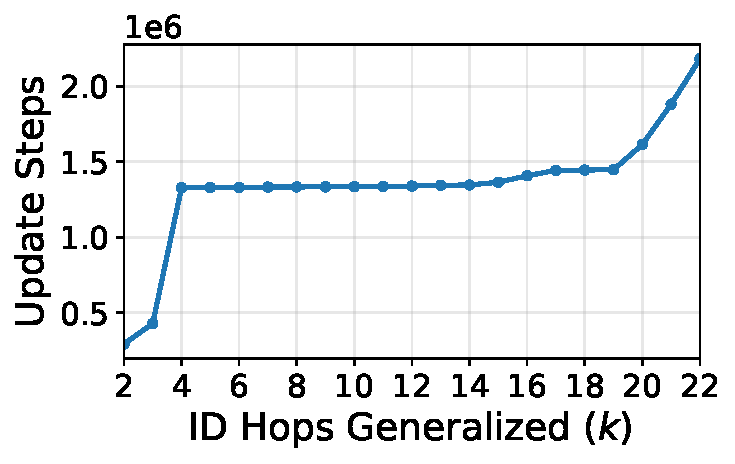
\includegraphics[width=0.33\textwidth]{images/curriculum_cumulative_updates_vs_hop.pdf}
%     \vspace{-0.6em}
%     \caption{Cumulative gradient updates required to first generalize to each hop complexity.}
%     \label{fig:curriculum-cumulative}
%     \vspace{-1.0em}
% \end{wrapfigure}

% % \paragraph{Phase transition from prolonged training to rapid learning.}
% We observe that models require a prolonged training phase to acquire low-hop tasks, after which they rapidly generalize to much more complex samples (Figure~\ref{fig:curriculum-cumulative}). 
% We illustrate this for the model trained with dynamic recurrence by plotting training steps against the compositional complexity achieved on in-distribution data.
% This suggests that the main difficulty lies in discovering the underlying compositional rule. 
% Once such a rule is internalized, the model can quickly extend it to samples of much higher complexity. 
% In Figure~\ref{fig:curriculum-cumulative} we observe how the model required over 1.3 million steps for grokking up to 4-hop train samples but was quickly able to learn up to 19-hop samples very few additional steps. Beyond that, for even more complex samples, while each new hop requires additional training steps to cross the 95\% threshold, the model still achieves strong generalization (\textgreater90\%) on hops 20, 21, and 22 within fewer than 8k extra steps per hop which is commensurate with the steps required for each additional hop from 4 through 19. By loading a trained checkpoint (20, say) and continuing training exclusively on 21-hop samples instead of the data mix consisting of samples from all previous stages in our curriculum, generalization over 90\% on the new split can be achieved in as little as 50 additional steps of training.

\section{Causal analysis of systematic generalization}
\label{app:causal}

We additionally perform a causal analysis using activation patching together with logit-lens decodability, and present the results in Figure~\ref{fig:causal}. In the figure, the color shading of each node indicates decodability: for the top row, how strongly the bridge entity $b$ is decoded at token position $r_1$, and for the bottom row, how strongly the target entity $t$ is decoded at position $r_2$, across effective depth. The thickness of the curved arrows shows causal strength measured by activation patching: we corrupt the first-hop prefix $(h, r_1)$, restore the clean activation at position $r_1$ at a given effective depth, and measure how much the final target prediction is recovered. We use the term “causal site” in the figure to denote the layer at position $r_1$ that exhibits the strongest causal effect under activation patching.

\begin{figure}[h]
    \centering
    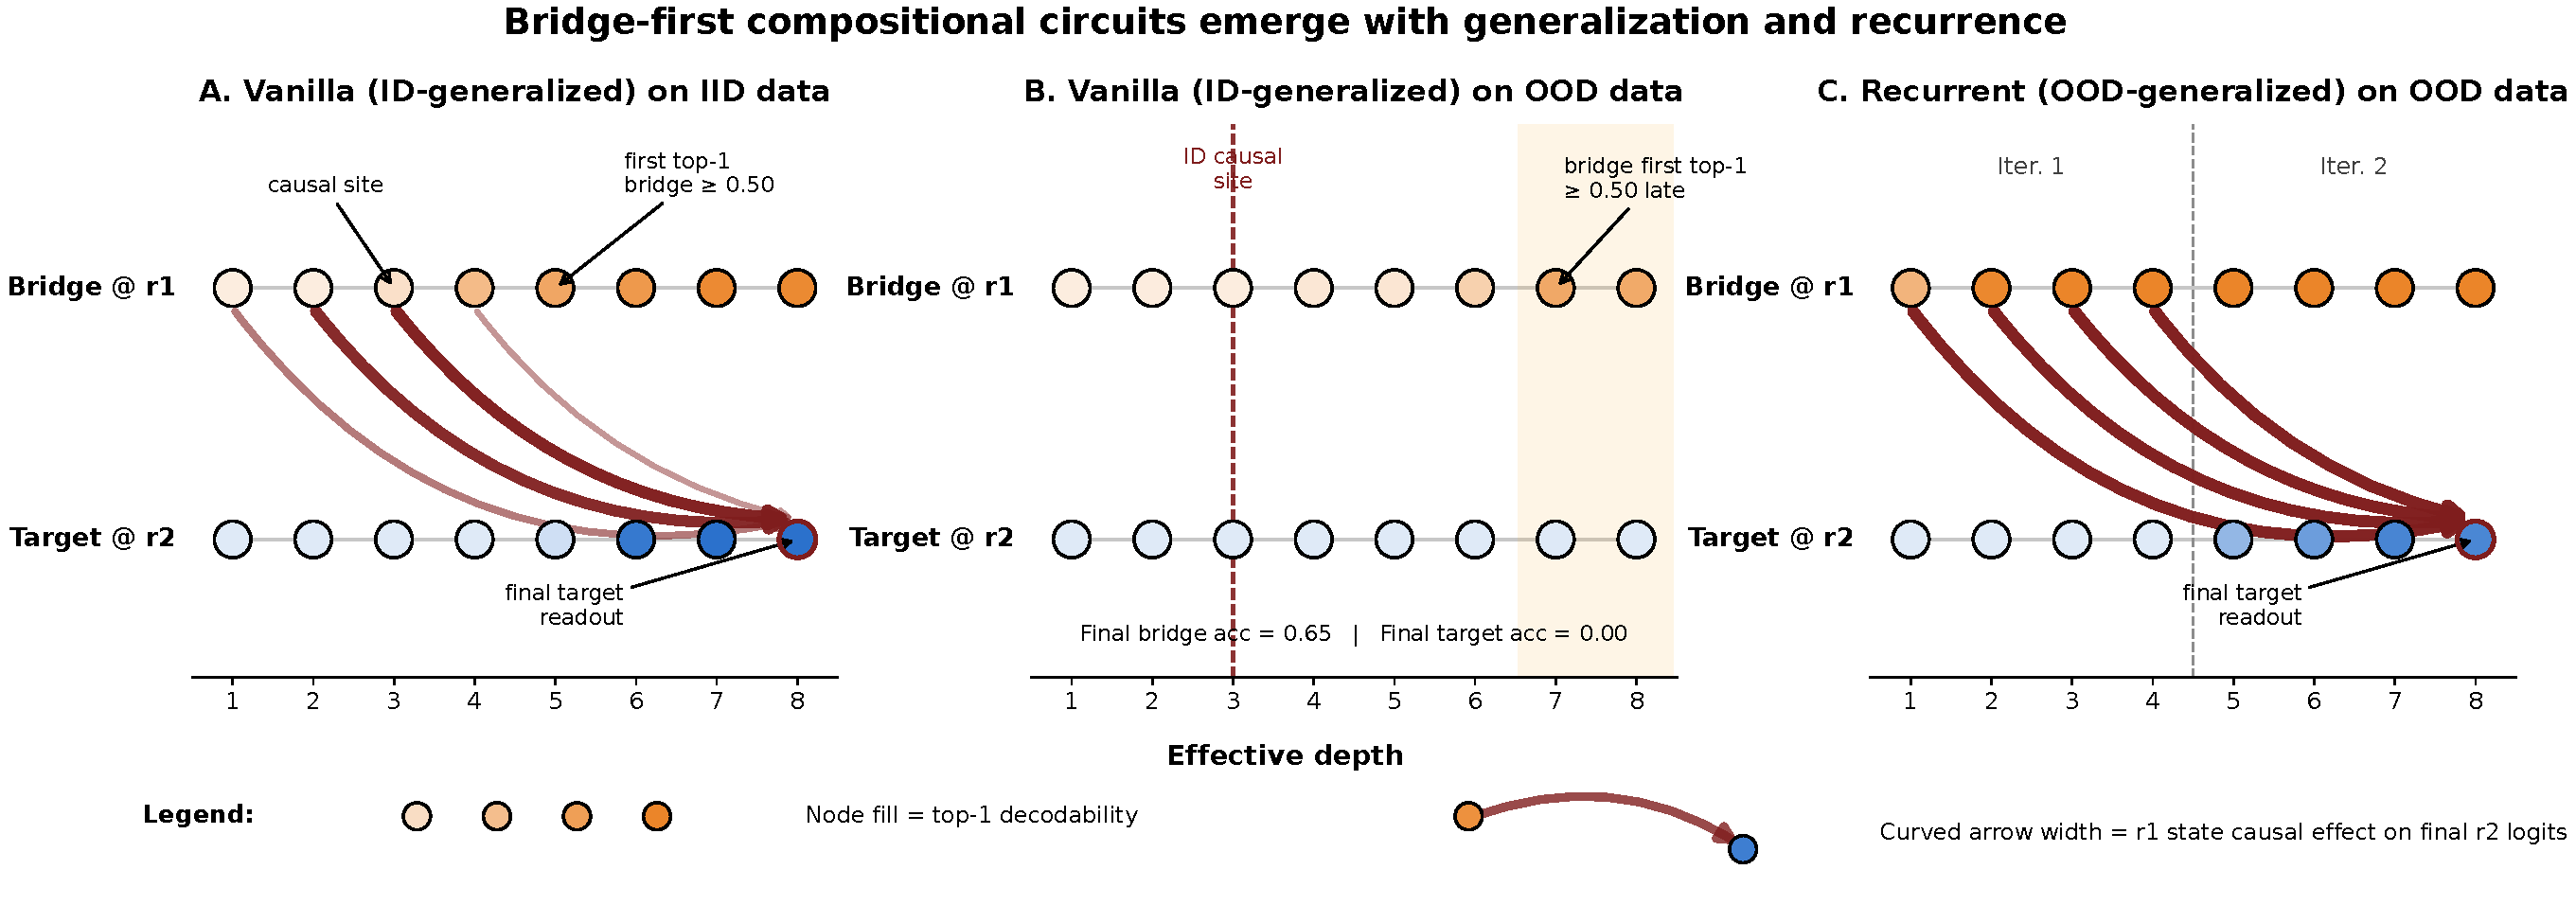
\includegraphics[width=\linewidth]{images/causal_analysis_for_paper.pdf}
    \caption{Bridge-mediated composition across effective depth in our systematicity setup.}
    \label{fig:causal}
\end{figure}

Panel A shows that, on ID data, the bridge becomes decodable at $r_1$ in shallow layers (layers 5), and these layers exhibit causal effects on the final answer prediction. Panel B shows that, on OOD data, the vanilla model only recovers the bridge at much deeper layers (layer 7+), and the target never becomes decodable. This suggests that the model can access the OOD first-hop rule only too late to use it for the second-hop composition. Panel C shows that the recurrent-depth model alleviates this issue: all layers in the first iteration at position $r_1$ show causal effects on the final answer prediction, and subsequent recurrent iterations can reuse the same parametric rule to complete the second-hop composition.

\section{Experiments with default initialization}
\label{app:default-init}

Here we report results obtained using the default Gaussian initialization for the \texttt{c\_proj} matrices, rather than the zero-initialization described in Section~\ref{sec:model-design}. As observed from Figure~\ref{fig:default-init-main}, the results are mixed across training runs, and increasing recurrence does not yield a clear or consistent pattern of improved ID or OOD generalization as well as robustness to latent overthinking. Only the model trained with $R=7$, hows strong signs of inference-time scaling and robustness to latent overthinking. In the case of the model trained with $R=5$, there is no OOD generalization with increased recurrence at inference-time. For most of the other runs, we see performance degradation due to latent overthinking.

\begin{figure}[h]
    \centering
    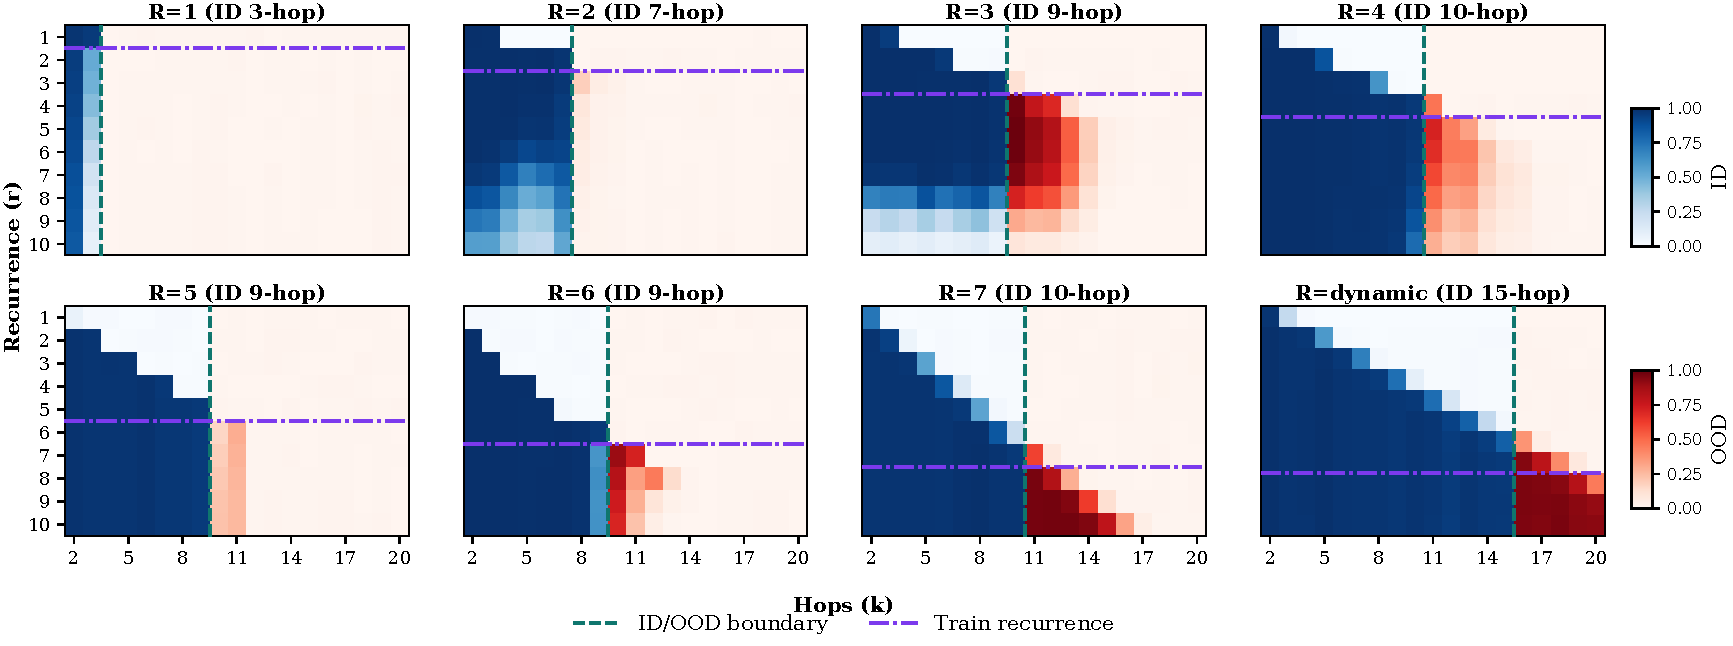
\includegraphics[width=\linewidth]{images/appendix_unstable_accuracy_region.pdf}
    \caption{Results with default initialization for training recurrences $R \in \{1,\dots,7\}$ and dynamic recurrence.}
    \label{fig:default-init-main}
\end{figure}

To further examine this instability, we train the $r=5$ model with five different random seeds. As shown in Figure~\ref{fig:default-init-r5-seeds}, the resulting behaviors vary substantially across seeds. Seed 1 is not affected by latent overthinking, but it also shows no evidence of inference-time scaling by solving harder compositional examples with increased recurrence. Seed 2 is likewise stable, but does exhibit scaling with additional recurrence. Seeds 3, 4, and 5 show varying degrees of inference-time scaling, but also experience performance degradation as recurrence increases, consistent with latent overthinking.

\begin{figure}[h]
    \centering
    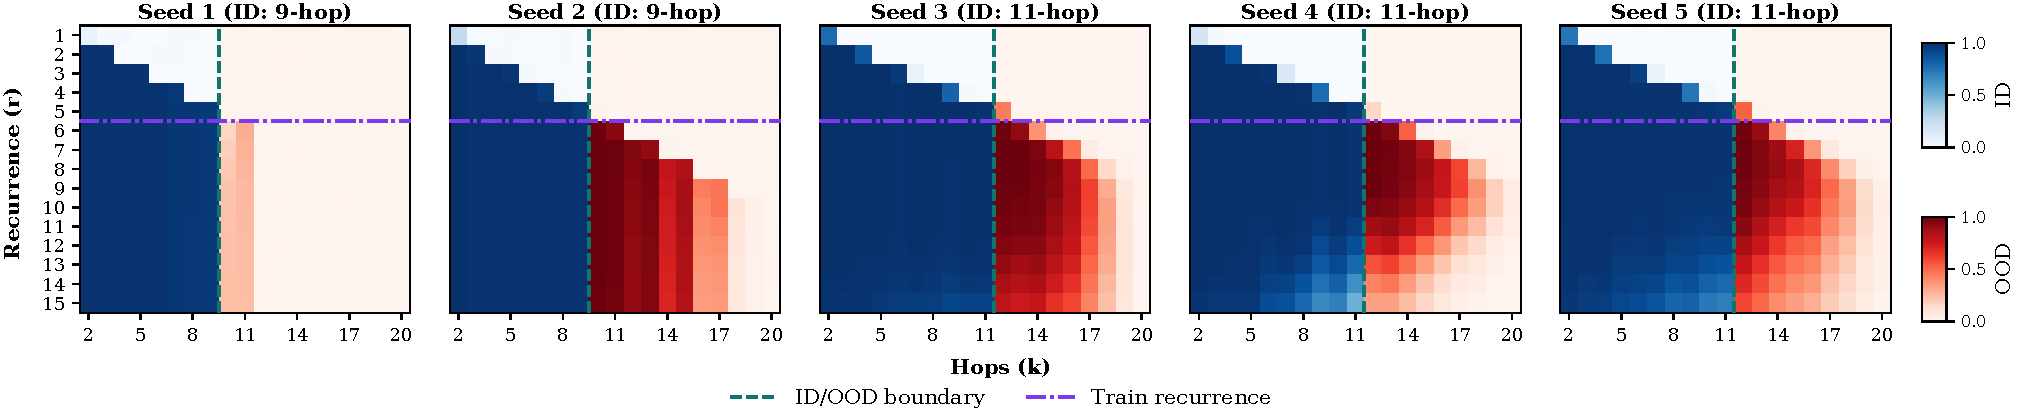
\includegraphics[width=\linewidth]{images/paper_unstable_r5.pdf}
    \caption{Five random-seed runs for the $R=5$ model with default initialization.}
    \label{fig:default-init-r5-seeds}
\end{figure}

\section{Experiments with larger vanilla transformers}
\label{app:isoflop_vanilla}

\begin{figure}[h]
    \centering 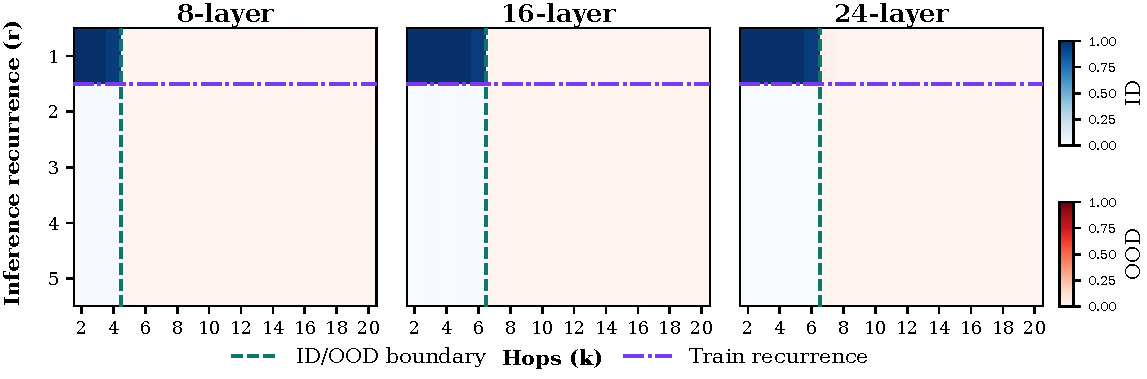
\includegraphics[width=0.6\linewidth]{images/paper_isoflop_accuracy_region_3panel.pdf}
    \caption{Depth extrapolation with larger vanilla transformers.}
    \label{fig:large_vanilla}
\end{figure}

We present additional results for larger vanilla transformers in Figure~\ref{fig:large_vanilla}. Specifically, we train 8-layer, 16-layer, and 24-layer vanilla transformers using the same setup as in Section~\ref{sec:exp_setup}. These results show that deeper vanilla models often achieve better ID generalization and can go beyond the 2-hop or 3-hop generalization observed in the 4-layer vanilla baseline. This is consistent with prior work showing that in-distribution generalization can improve with greater depth in vanilla transformers [1]. However, their ID generalization remains weaker than recurrent-depth models with the same effective depth. More importantly, the vanilla models still do not exhibit OOD generalization to more complex samples, and they lack the flexibility to scale computation according to sample complexity in the way recurrent-depth models can.

\section{Additional experiments with matched-hop data}
\label{app:matched_data}

We provide additional extrapolation results for models with different loop iterations trained on matched-hop data in Figure~\ref{fig:matched_large}. From top to bottom, the rows show results for models trained on data up to 8-hop, 10-hop, and 12-hop, while each column corresponds to a different training recurrence setting. The general trend is consistent with Figure~\ref{fig:extrapolation2}: models trained with higher recurrence achieve stronger OOD generalization through inference-time scaling.

\begin{figure}[h]
    \centering
    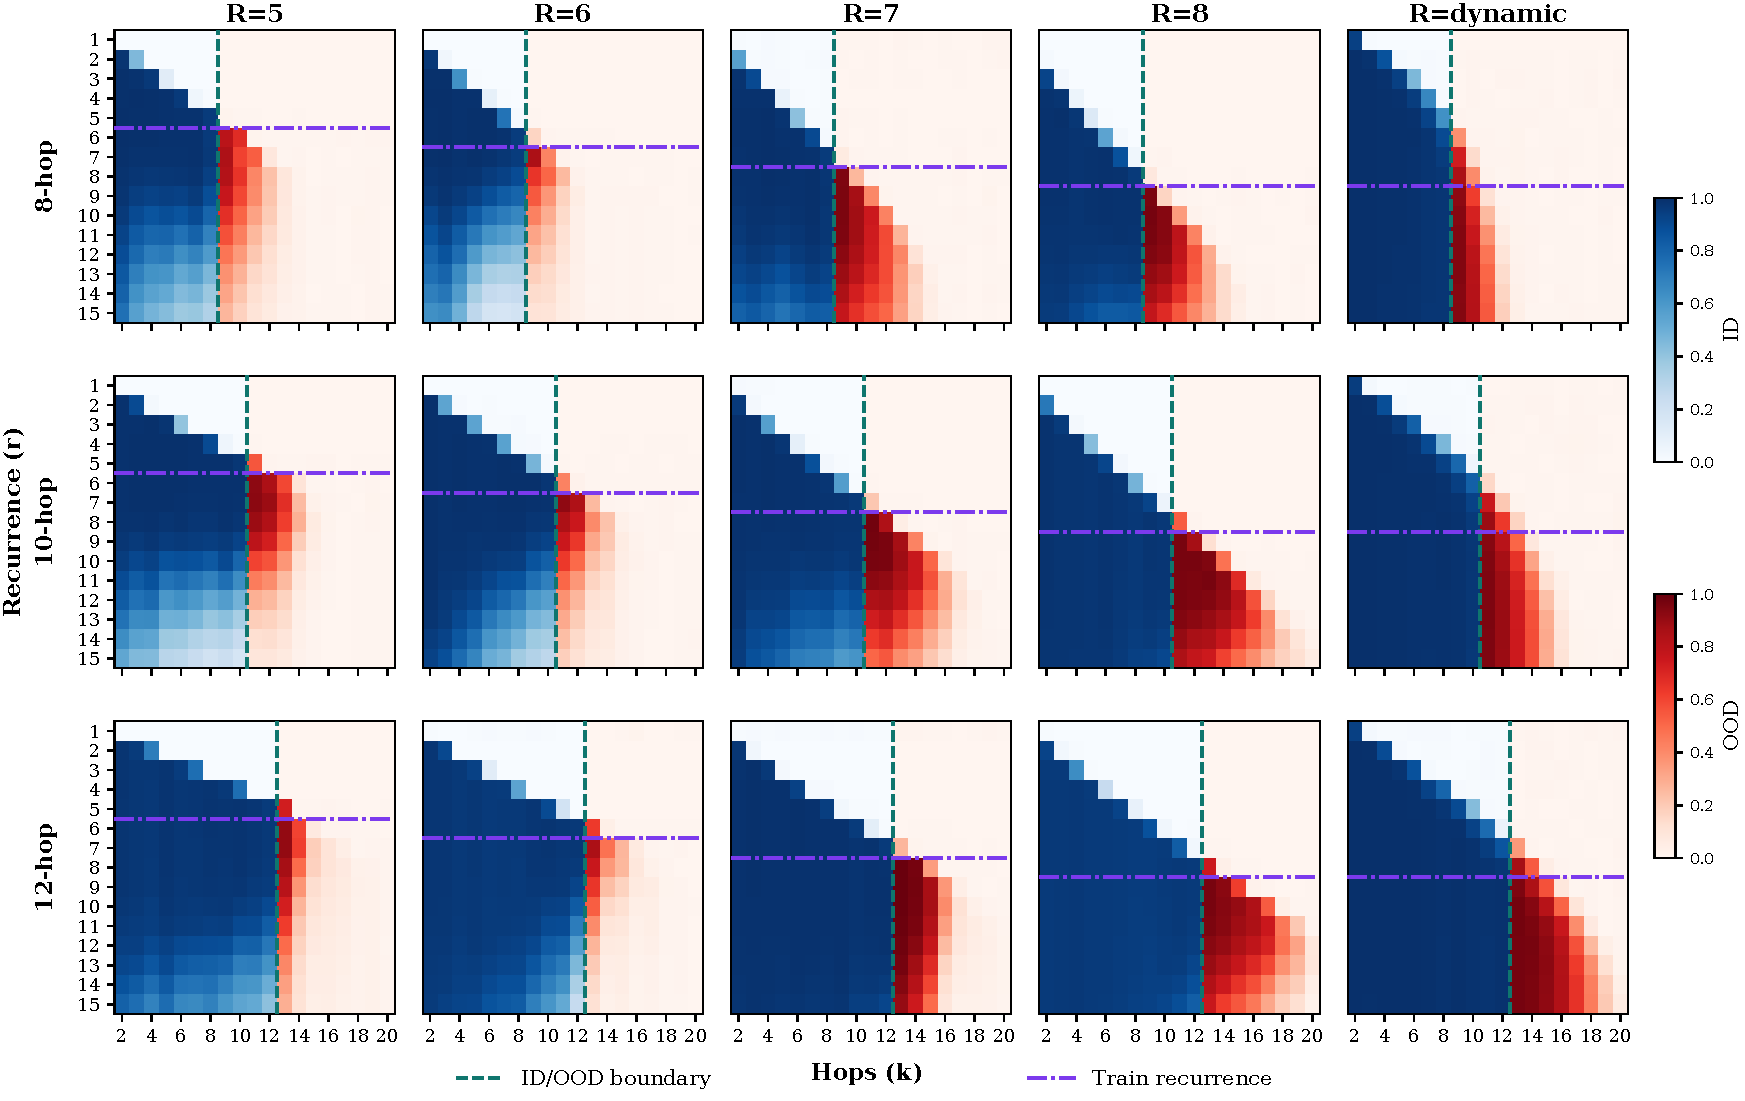
\includegraphics[width=\linewidth]{images/matched_data_3row.pdf}
    \caption{Matched-data experiments with varying train-time recurrence.}
    \label{fig:matched_large}
\end{figure}


% \section{Comparison with KL-divergence-only halting}\label{app:halting}

% \begin{figure}[h]
%     \centering
%     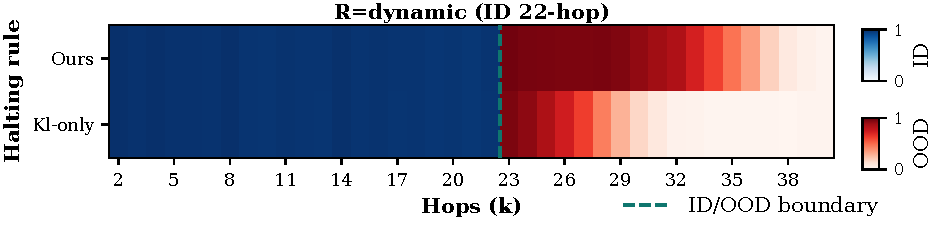
\includegraphics[width=0.6\linewidth]{images/dynamic_adaptive_rows_only.pdf}
%     \caption{Comparison of adaptive halting based on KL-divergence and entropy (ours) versus KL-divergence alone \citep{geiping2025scaling}. The figure shows accuracy across hop complexity for the dynamic-recurrence model using the joint criterion (ours) and the KL-only criterion (KL-only).}
%     \label{fig:dynamic-adaptive-rows}
% \end{figure}

% We also experiment with a KL-divergence-only halting criterion, similar to \citet{geiping2025scaling}, but find that it often halts recurrence prematurely ~\ref{fig:adaptive-iterations-vs-hops}. While the output distribution may change very little across iterations, the entropy is still high, indicating that the model remains uncertain despite this apparent convergence. We compare results in our dynamic model using both methods in Figure~\ref{fig:dynamic-adaptive-rows}. In our setting, combining KL divergence with entropy therefore provides a more reliable halting signal and yields the best overall results.

\section{Results with different random seeds}\label{app:seeds}

We run our fixed-recurrence models on 2 separate random seed initializations (including the run shown in Figure~\ref{fig:extrapolation}) and with to 40 recurrent iterations at inference time. On both runs, we notice the same general trend of increasing ID and OOD generalization with higher train-time recurrence as well as issues due to latent overthinking (with the sole exception being the model trained with $r=8$ in the second run). The results are presented in Figures~\ref{fig:seed1} \&~\ref{fig:seed2}.

\begin{figure}[h]
    \centering
    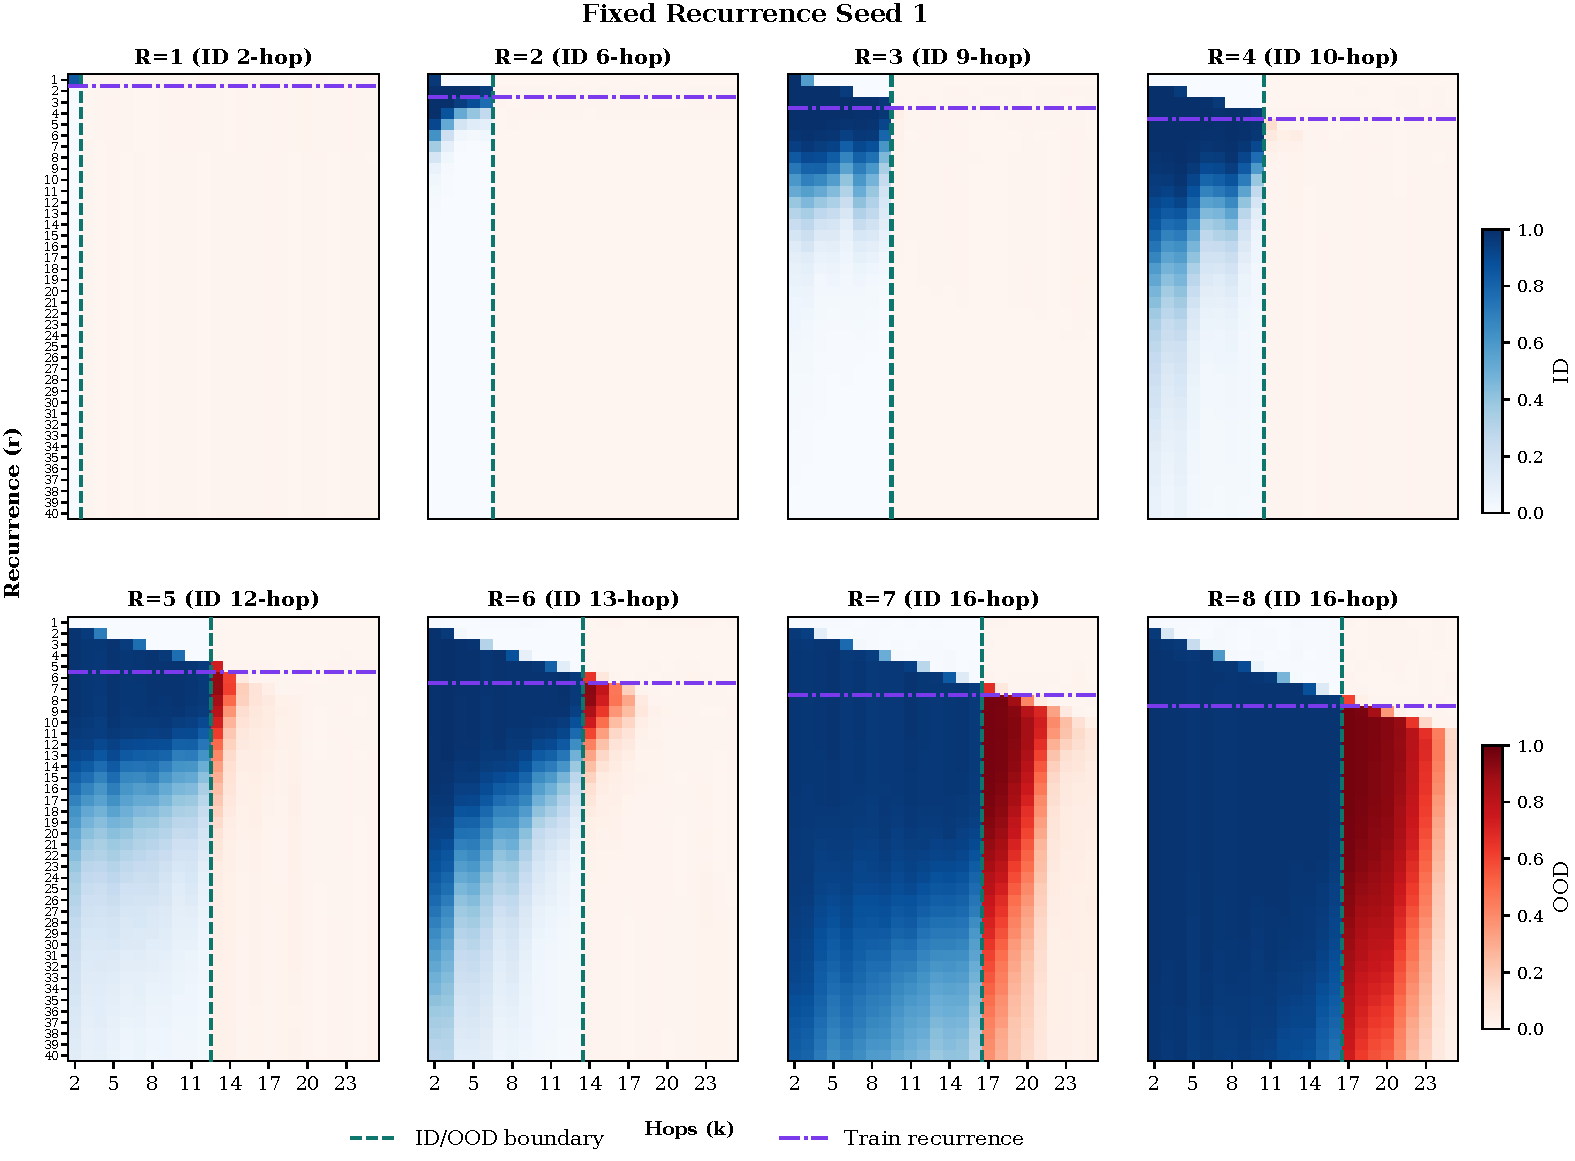
\includegraphics[width=0.9\linewidth]{images/main_results_42_accuracy_region_fixed_2x4.pdf}
    \caption{Results for Seed 1.}
    \label{fig:seed1}
\end{figure}

\begin{figure}[h]
    \centering
    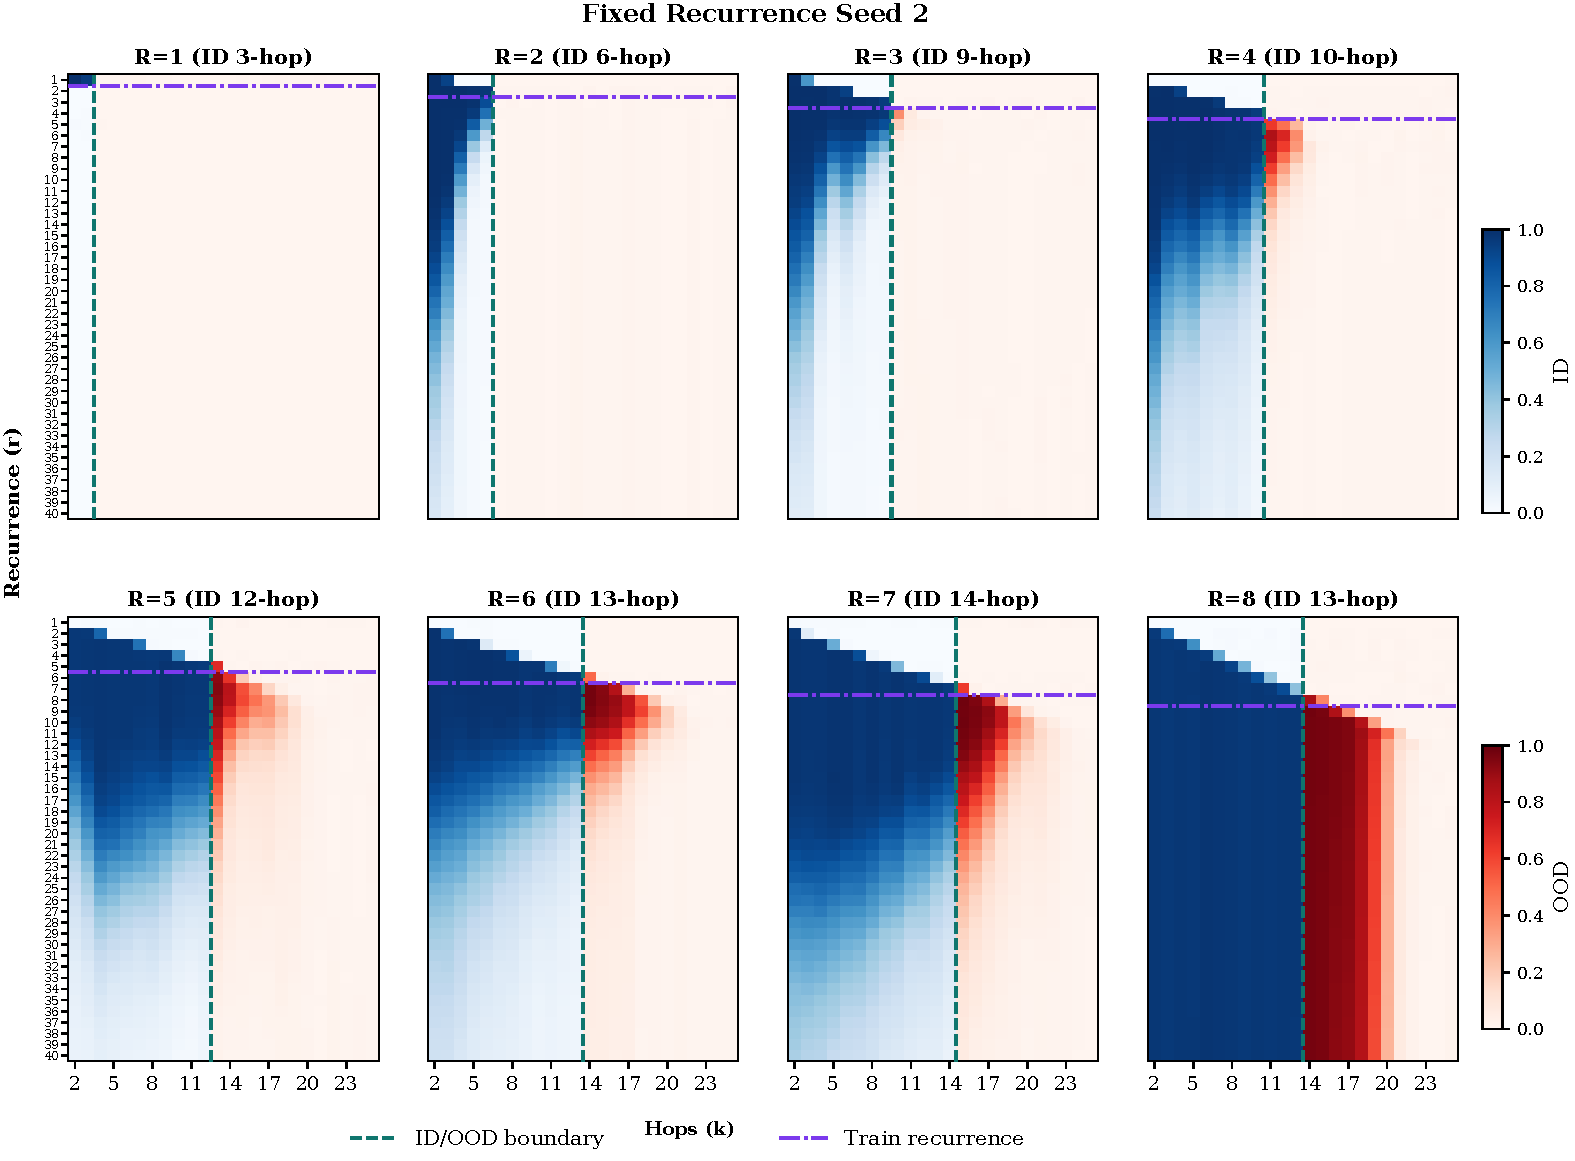
\includegraphics[width=0.9\linewidth]{images/main_results_222_accuracy_region_fixed_2x4.pdf}
    \caption{Results for Seed 2.}
    \label{fig:seed2}
\end{figure}

We similarly plot the performance of the dynamic recurrence model across three different seeds and observe a generally high ID generalization and OOD extrapolation. Across all seeds, the dynamic recurrence model is robust to the latent overthinking phenomenon and adaptive halting ($r^*$) works reliably to stop recurrence when not necessary.

\begin{figure}[h]
    \centering
    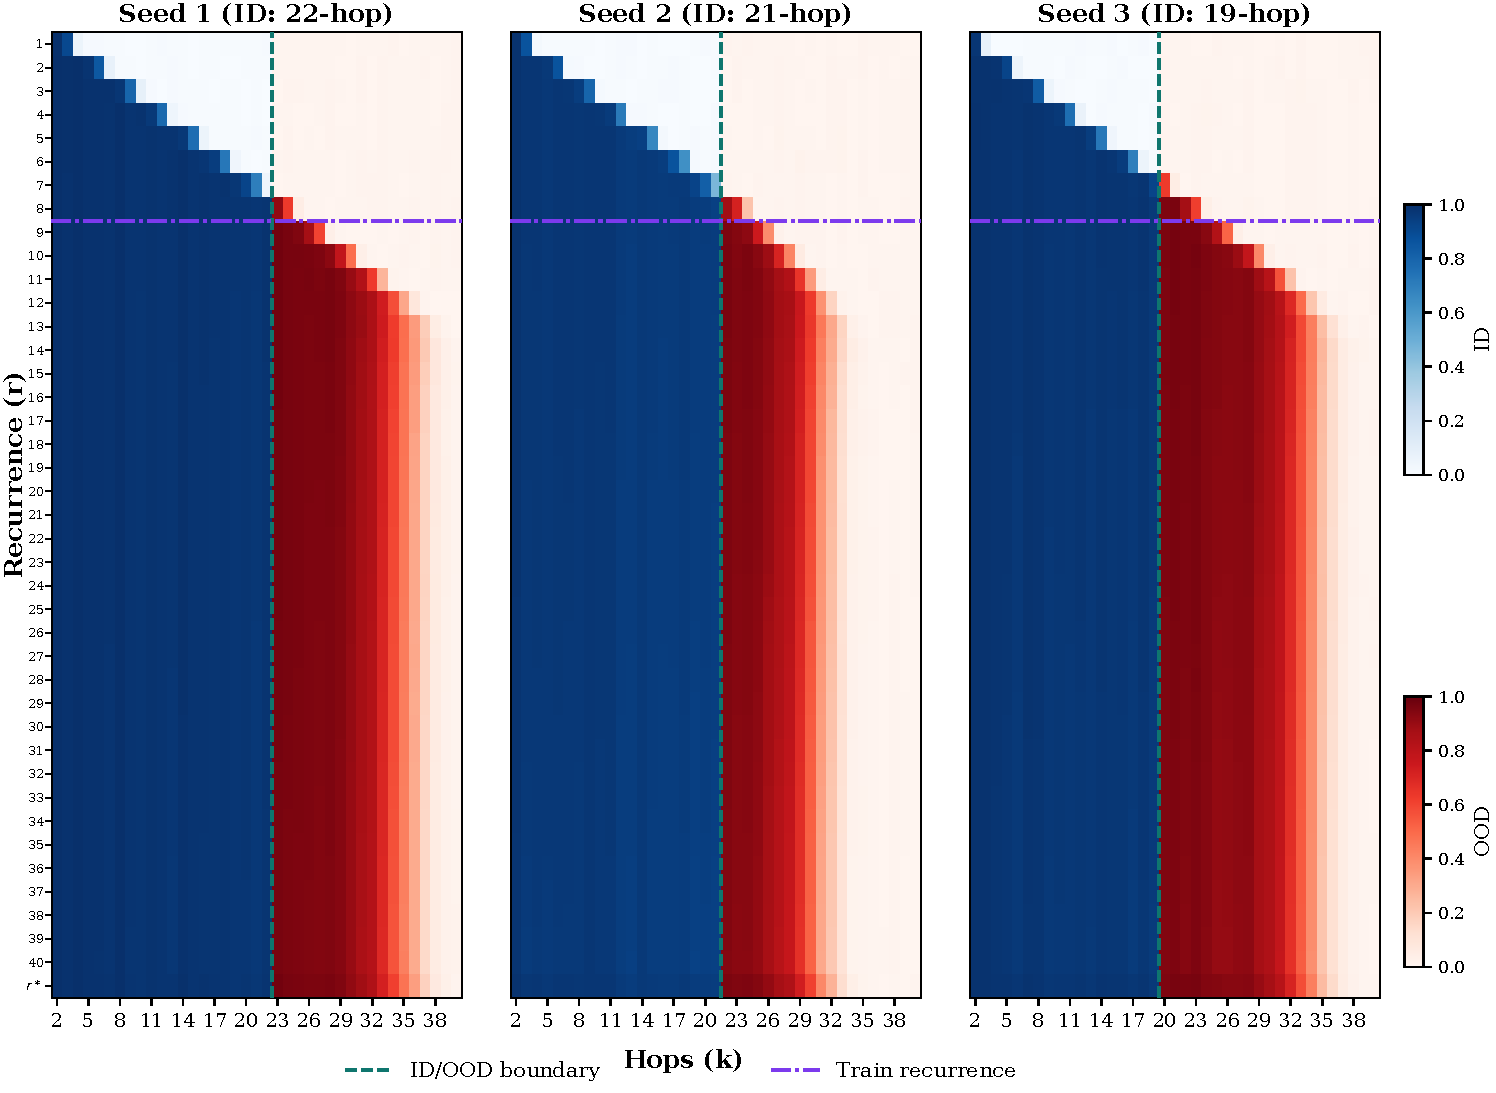
\includegraphics[width=0.7\linewidth]{images/dynamic_seeds_accuracy_region_dynamic_1x3.pdf}
    \caption{Dynamic recurrence with 3 difference random seed initializations.}
    \label{fig:dynamic_seeds}
\end{figure}

\section{Extrapolation with varying model size and dynamic recurrence}\label{app:ratios}

We carry out additional experiments to study how extrapolation behavior changes with model size and with training recurrence in our dynamic recurrence setting. In addition to our default 4-layer model, we train larger models with 6 and 8 layers. We also vary the maximum recurrence used during dynamic-recurrence training, considering settings with maximum train-time recurrence of 8, 12, and 16. For these, the recurrence at each training iteration is sampled from a Poisson distribution with means 4, 6, and 8 respectively, with a minimum recurrence of 2 in all cases.

\begin{figure}[h]
    \centering
    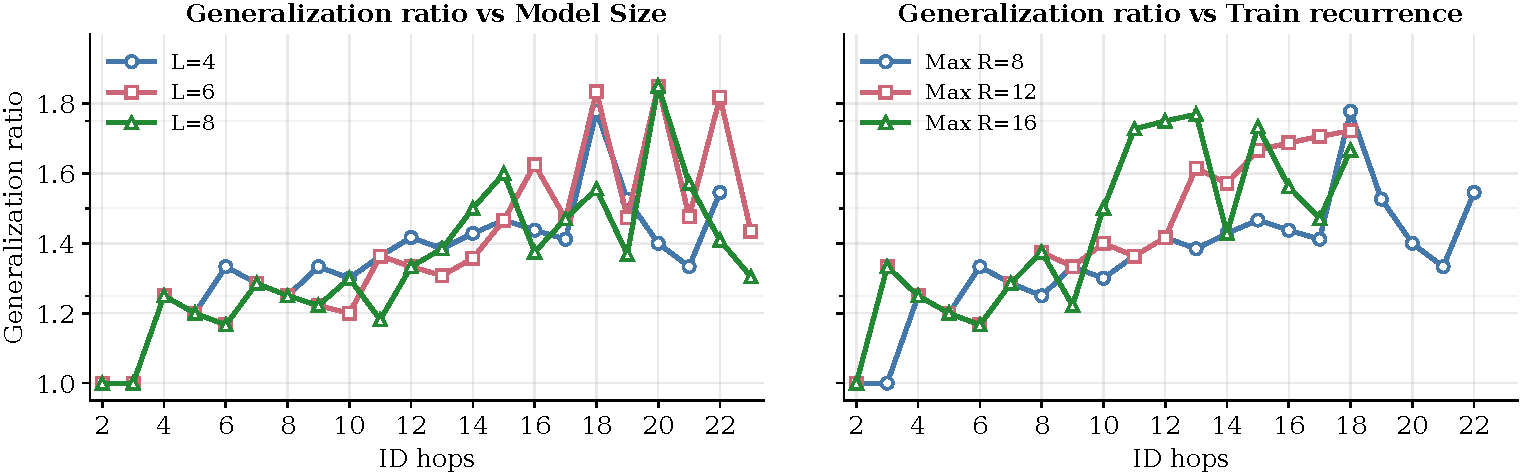
\includegraphics[width=\linewidth]{images/generalization_ratio_two_panel.pdf}
    \caption{Generalization ratio with changing model size and train recurrence.}
    \label{fig:ratios}
\end{figure}

To summarize extrapolation under these settings, we plot the \emph{generalization ratio}, defined as the maximum hop complexity to which a model can generalize with at least 60\% accuracy with inference-time scaling, divided by the maximum hop complexity that the model has generalized to during training. This can be viewed as the ratio of maximum OOD generalization to maximum ID generalization. A ratio of 1 indicates no extrapolation beyond the level reached during training, while larger values indicate successful extrapolation to more complex compositions at test time.

Figure~\ref{fig:ratios} shows that models initially begin with a ratio close to 1. In particular, when models have only generalized to 2-hop composition during training, they do not yet extrapolate to more complex samples. As training progresses and the models have seen more complex compositions through our curriculum learning setup, the ratio increases. However, across both model-size variations and different maximum train-time recurrence settings, we do not observe a clear or consistent trend indicating that either larger models or larger train-time recurrence systematically improves this ratio. 

% \section{Experiments with default initialization}
% \label{app:default-init}

% \begin{figure}[h]
%     \centering
%     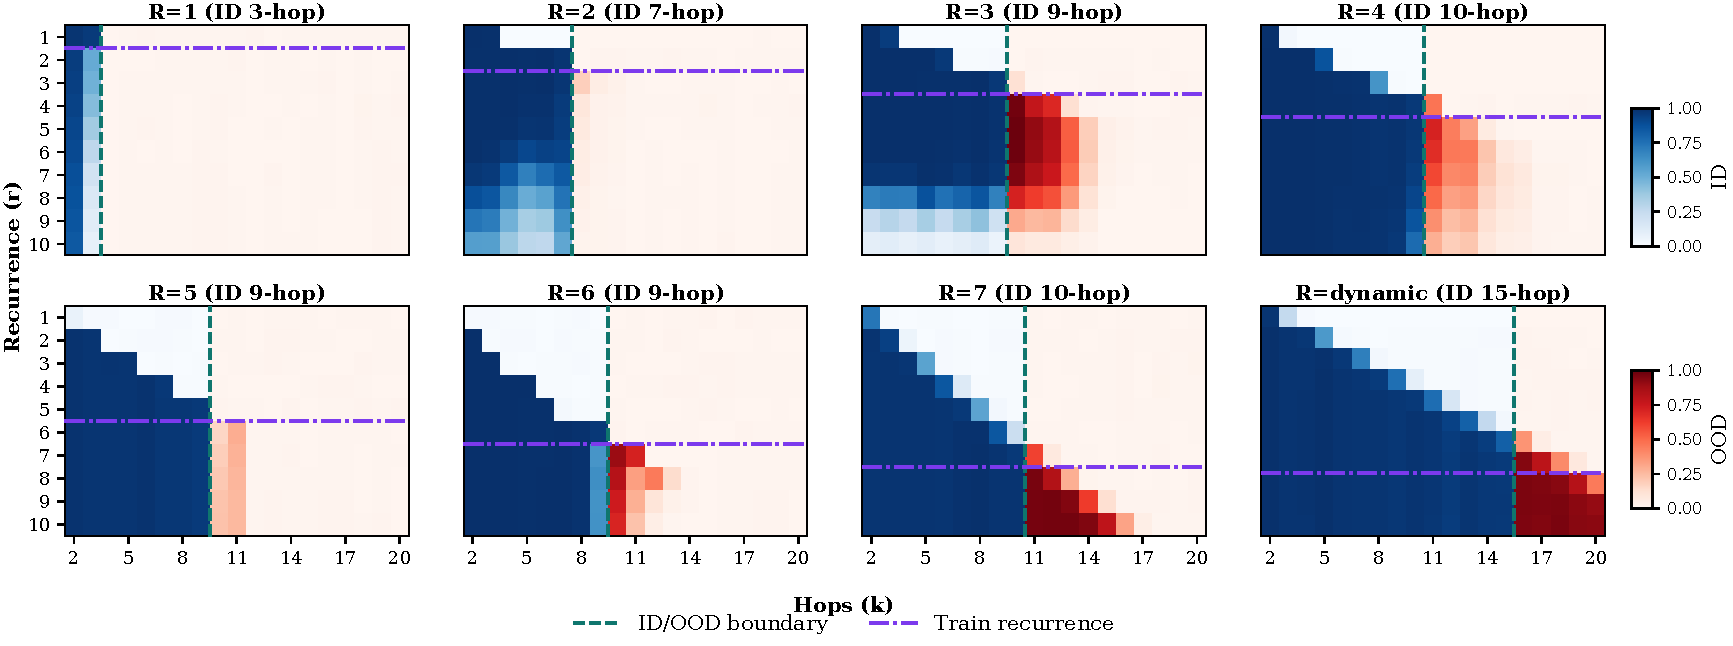
\includegraphics[width=\linewidth]{images/appendix_unstable_accuracy_region.pdf}
%     \caption{Results with default initialization for training recurrences $R \in \{1,\dots,7\}$ and dynamic recurrence.}
%     \label{fig:default-init-main}
% \end{figure}

% Here we report results obtained using the default Gaussian initialization for the \texttt{c\_proj} matrices, rather than the zero-initialization described in Section~\ref{sec:model-design}. As observed from Figure~\ref{fig:default-init-main}, the results are mixed across training runs, and increasing recurrence does not yield a clear or consistent pattern of improved ID or OOD generalization as well as robustness to latent overthinking. Only the model trained with $R=7$, hows strong signs of inference-time scaling and robustness to latent overthinking. In the case of the model trained with $R=5$, there is no OOD generalization with increased recurrence at inference-time. For most of the other runs, we see performance degradation due to latent overthinking.

% \begin{figure}[h]
%     \centering
%     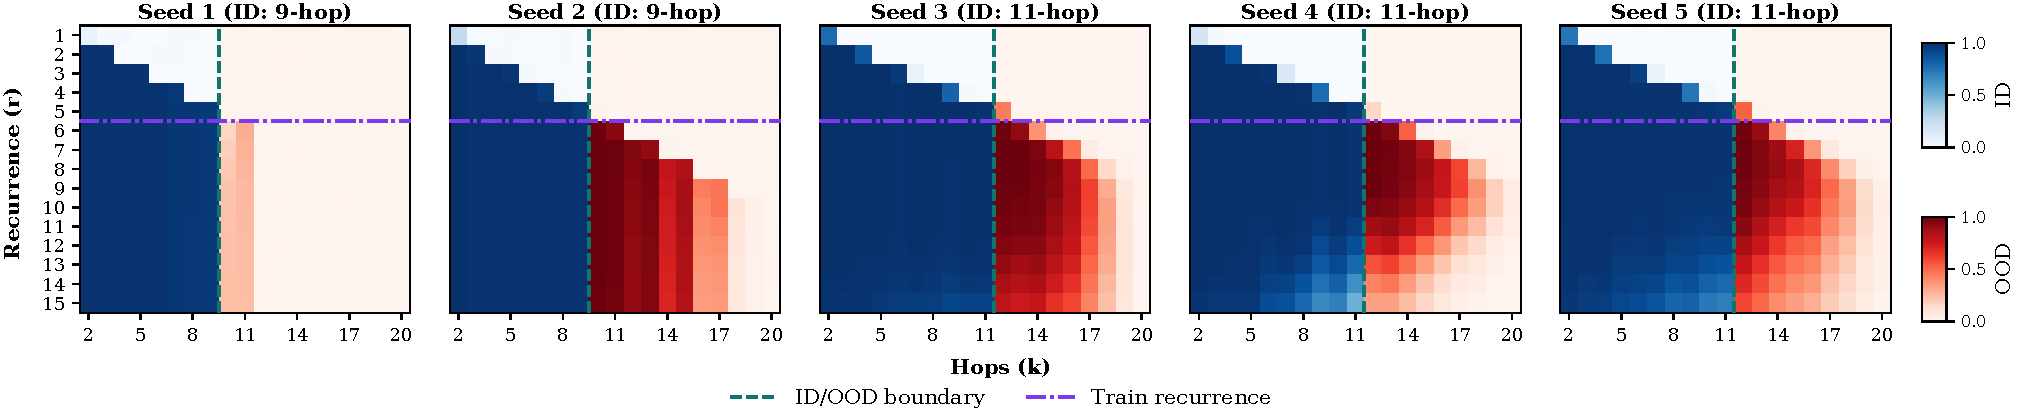
\includegraphics[width=\linewidth]{images/paper_unstable_r5.pdf}
%     \caption{Five random-seed runs for the $R=5$ model with default initialization.}
%     \label{fig:default-init-r5-seeds}
% \end{figure}

% To further examine this instability, we train the $r=5$ model with five different random seeds. As shown in Figure~\ref{fig:default-init-r5-seeds}, the resulting behaviors vary substantially across seeds. Seed 1 is not affected by latent overthinking, but it also shows no evidence of inference-time scaling by solving harder compositional examples with increased recurrence. Seed 2 is likewise stable, but does exhibit scaling with additional recurrence. Seeds 3, 4, and 5 show varying degrees of inference-time scaling, but also experience performance degradation as recurrence increases, consistent with latent overthinking.

\section{Illusion of very deep composition through shortcuts}
\label{app:shortcut-effects}

Prior to adopting the permutation-based dataset construction described in Appendix~\ref{app:permutation}, we observed what appeared to be very deep compositional generalization. As shown in Figure~\ref{fig:shortcut2}, models trained on ID examples up to 40 hops achieved strong OOD performance even at 80 hops for models with $R=4$, $R=8$, and dynamic recurrence. This indicates that the model is able to resolve multiple hops or compositions in a single layer. To inspect this closely, we perform a causal activation-patching analysis. We first select a clean 60-hop test example whose relation sequence ends in a particular suffix, and a second random example of the same hop type. We then run both examples through the model and cache their hidden states. Next, for each token position and each recurrent iteration-layer location (as well as the embedding layer), we replace the hidden state in the clean run with the corresponding hidden state from the random run, and measure the resulting change in the logit margin of the correct final answer. Figure~\ref{fig:shortcut1-deltas} visualizes this change relative to the clean run.

\begin{figure}[h]
    \centering
    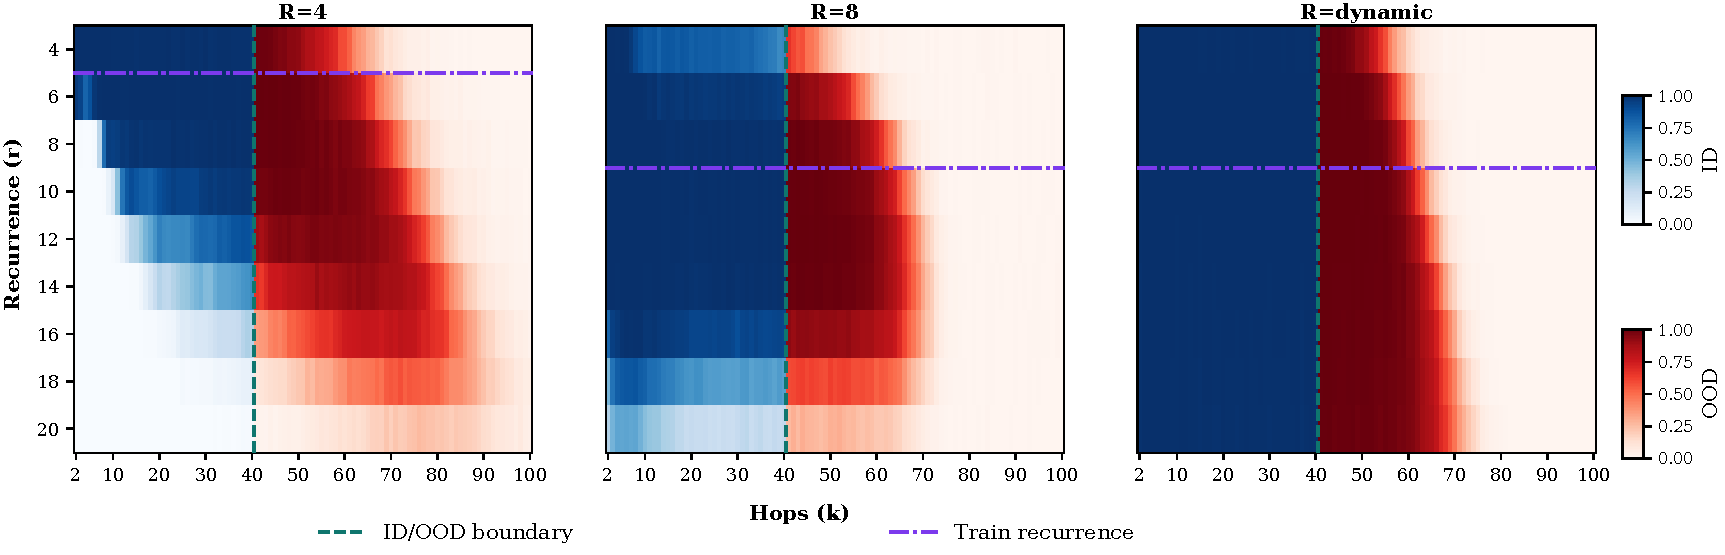
\includegraphics[width=0.8\linewidth]{images/shortcut2.pdf}
    \caption{Apparent deep compositional generalization in the pre-permutation dataset.}
    \label{fig:shortcut2}
\end{figure}

This analysis reveals that the model is not solving the full compositional chain. Instead, the strongest causal effects are concentrated on a short suffix of the relation sequence. The final tail entity can often be inferred from trailing relations alone, without explicitly retrieving the intermediate entities. The model learns a shallow mapping from a suffix of the relation sequence to the answer, rather than performing full multi-hop composition. These observations motivate the permutation-based knowledge graph introduced in Appendix~\ref{app:permutation}. Under that construction, each relation acts as a permutation over entities, so the correct final entity cannot be recovered from a short suffix alone, and the model must compose the full sequence of relations to solve the task.

\begin{figure}[h]
    \centering
    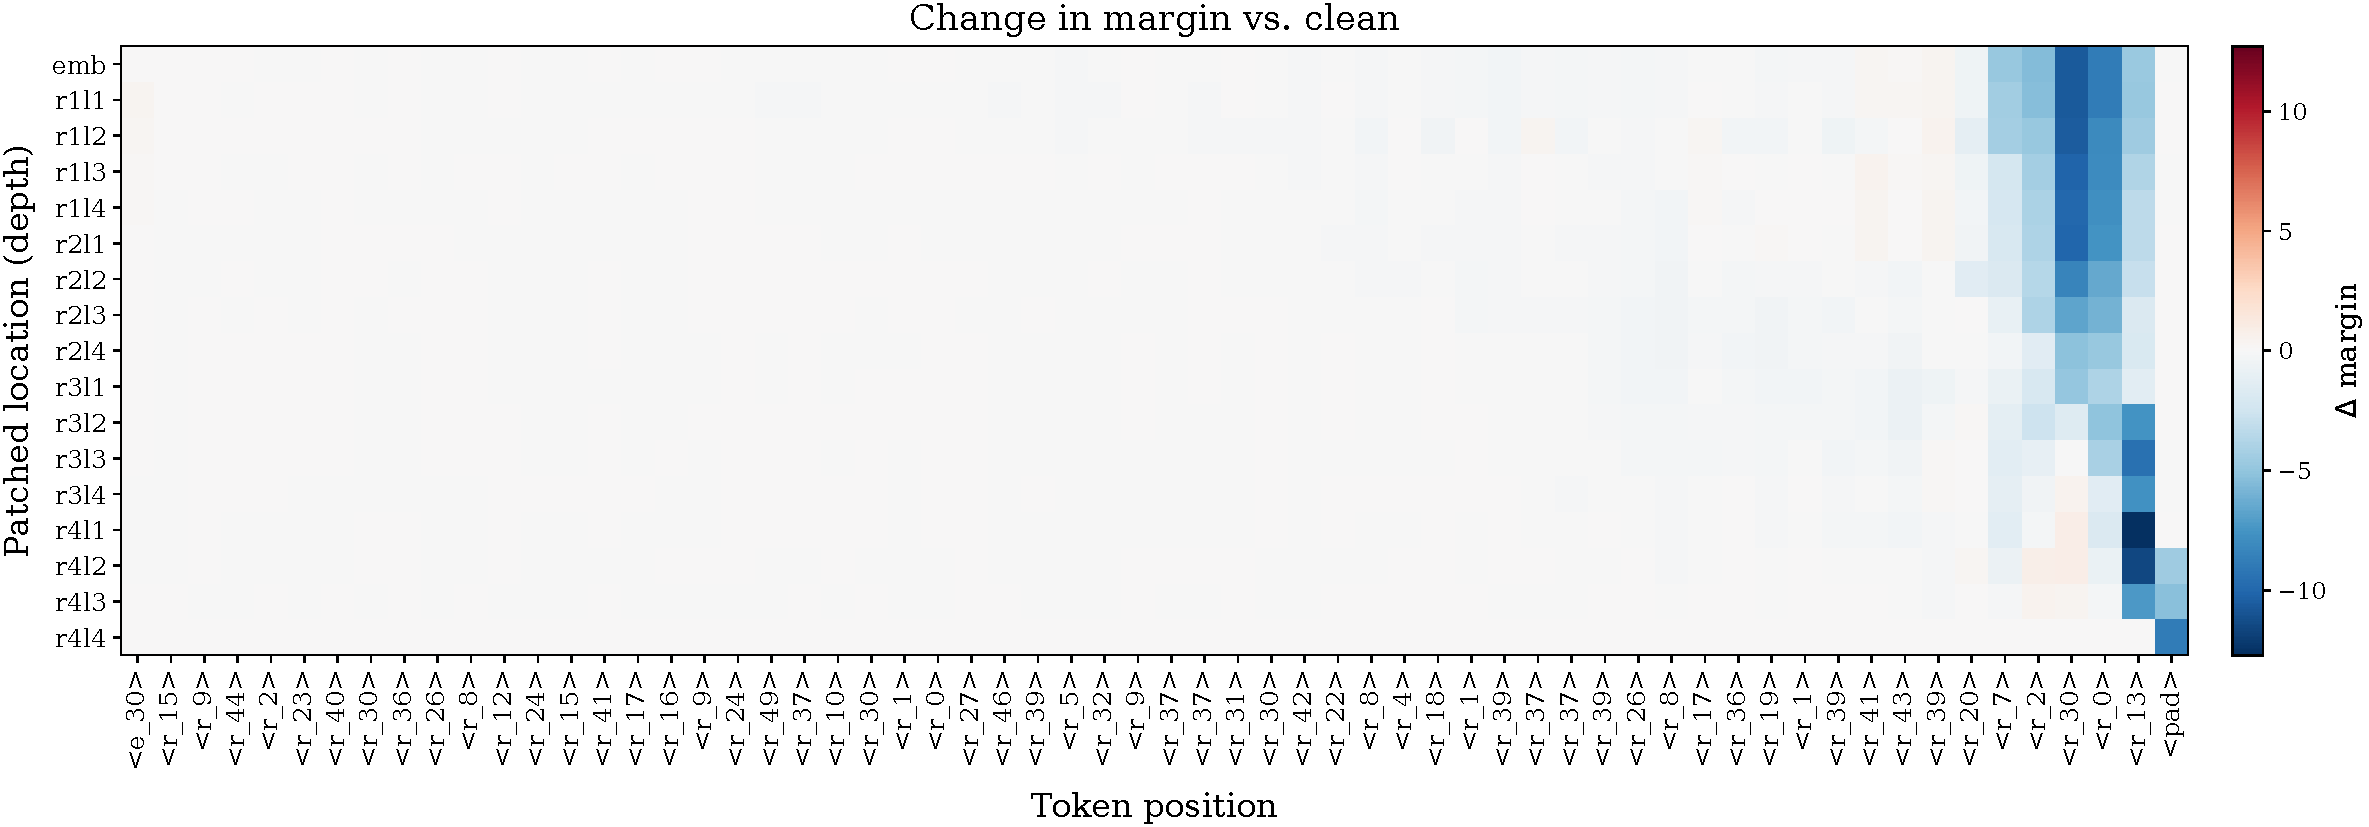
\includegraphics[width=0.9\linewidth]{images/shortcut1_deltas.pdf}
    \caption{Activation-patching analysis on a 60-hop example. Each cell shows the change in logit margin for the correct answer, relative to the clean run, after replacing a single hidden state in the clean example with the corresponding hidden state from a random 60-hop example. Large changes are concentrated towards the end of the relation sequence, indicating shortcut-based prediction rather than genuine multi-hop retrieval.}
    \label{fig:shortcut1-deltas}
\end{figure}
